\documentclass{standalone}
\usepackage{tikz}
\usetikzlibrary{patterns, positioning}
\usepackage[sfdefault]{ClearSans} %% option 'sfdefault' activates Clear Sans as the default text font
\usepackage[T1]{fontenc}

\begin{document}
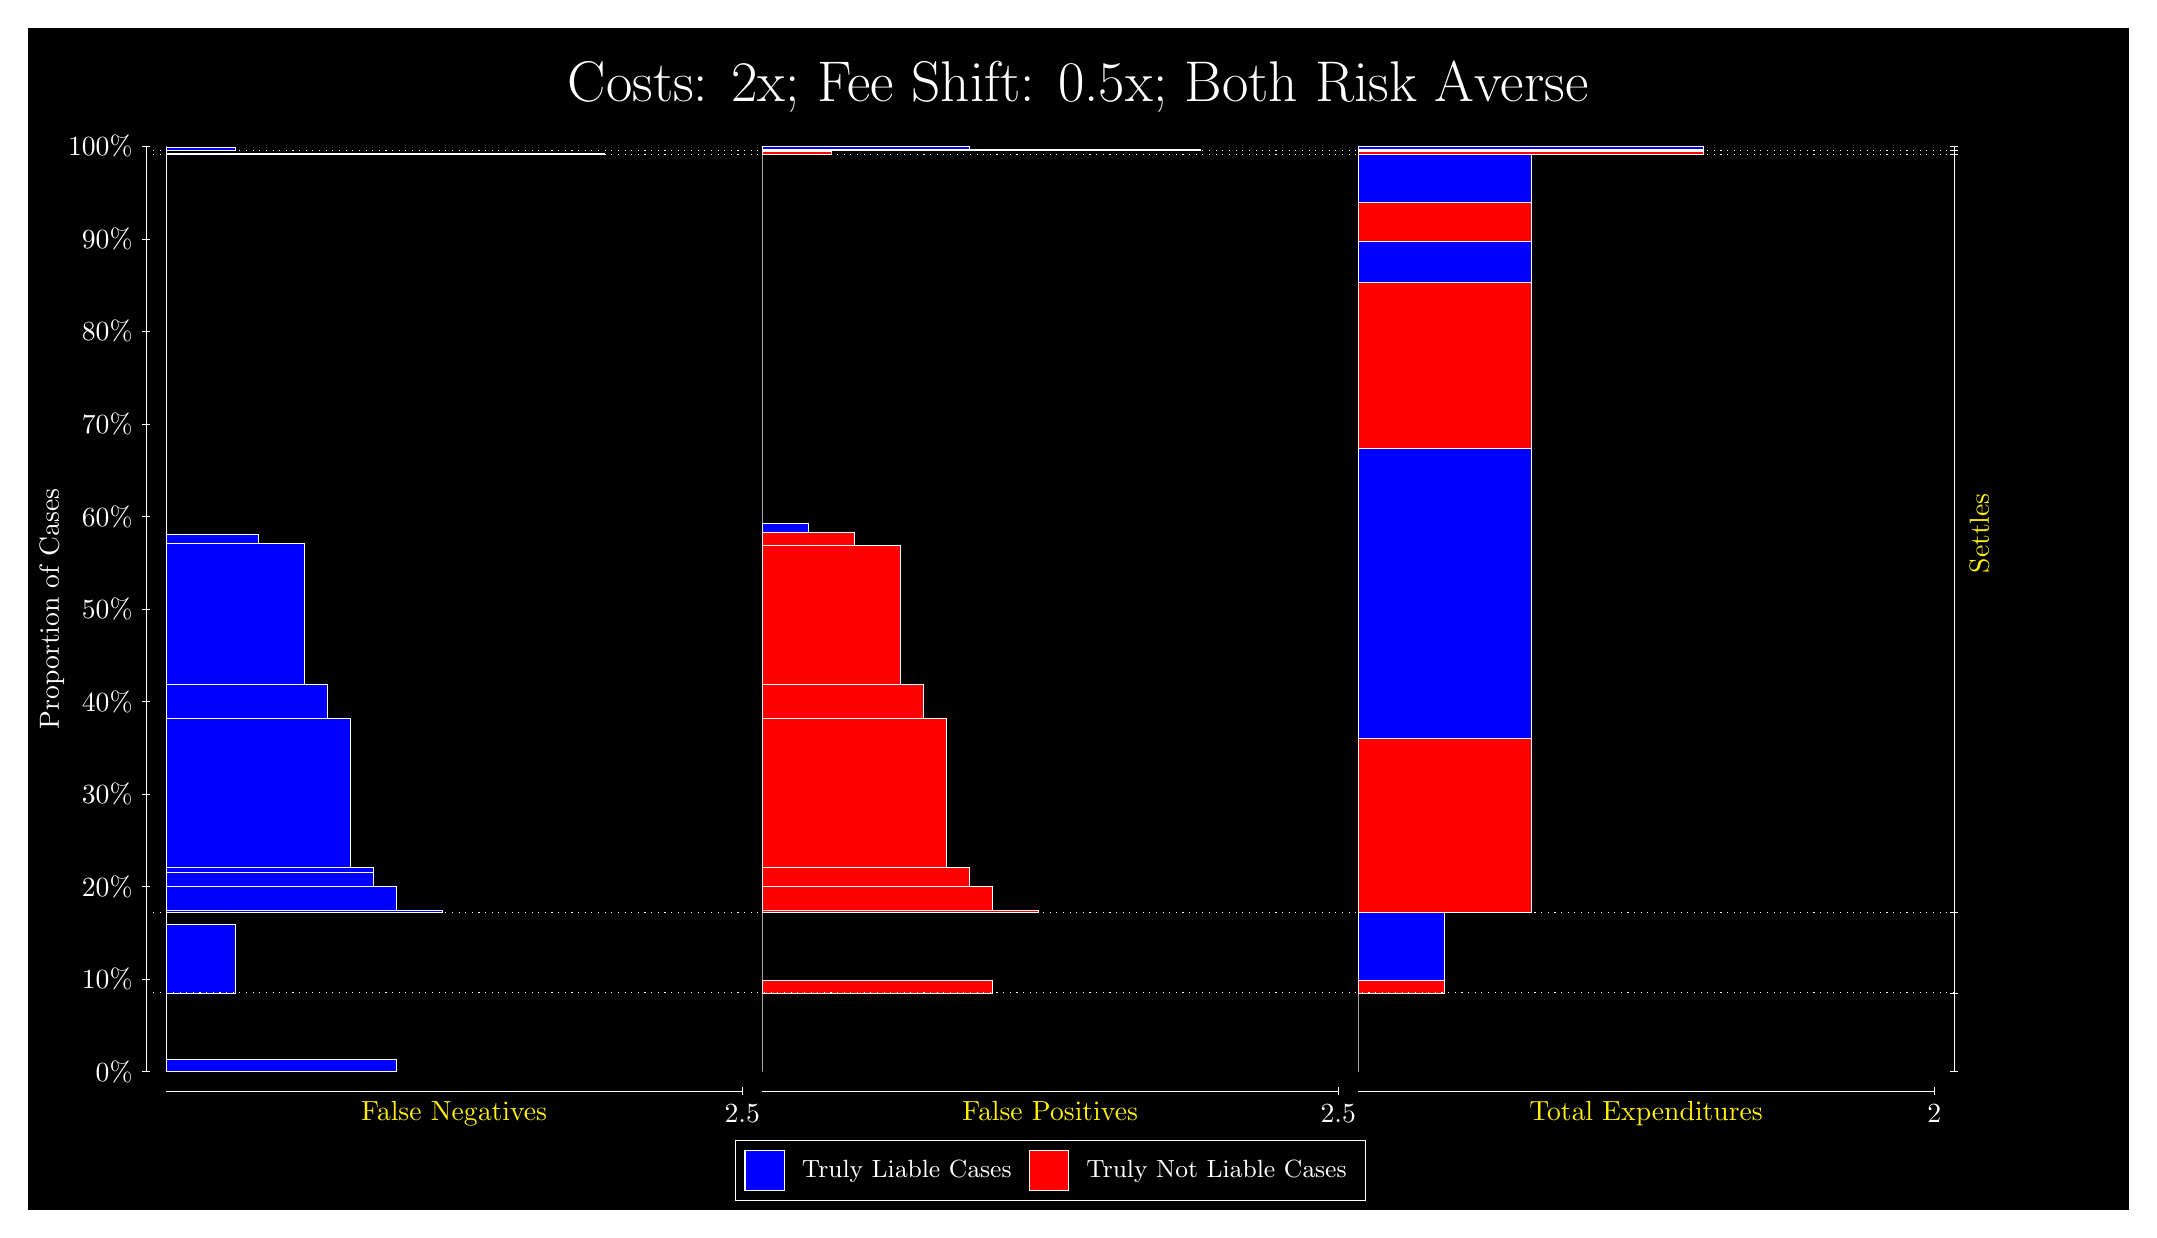
\begin{tikzpicture}
\draw[fill=black] (0,0) rectangle (26.667,15);
\draw[text=white] (0,13.5) rectangle (26.667,15) node[midway] {\huge Costs: 2x; Fee Shift: 0.5x; Both Risk Averse};
\draw[white, very thin] (1.5,1.75) -- (1.5,13.5);
\node[rotate=90, text=white, anchor=center] at (0.3, 7.625) {Proportion of Cases};
\draw[white, very thin] (1.45,1.75) -- (1.55,1.75);
\node[text=white, anchor=east] at (1.45, 1.75) {0\%};
\draw[white, very thin] (1.45,2.925) -- (1.55,2.925);
\node[text=white, anchor=east] at (1.45, 2.925) {10\%};
\draw[white, very thin] (1.45,4.1) -- (1.55,4.1);
\node[text=white, anchor=east] at (1.45, 4.1) {20\%};
\draw[white, very thin] (1.45,5.275) -- (1.55,5.275);
\node[text=white, anchor=east] at (1.45, 5.275) {30\%};
\draw[white, very thin] (1.45,6.45) -- (1.55,6.45);
\node[text=white, anchor=east] at (1.45, 6.45) {40\%};
\draw[white, very thin] (1.45,7.625) -- (1.55,7.625);
\node[text=white, anchor=east] at (1.45, 7.625) {50\%};
\draw[white, very thin] (1.45,8.8) -- (1.55,8.8);
\node[text=white, anchor=east] at (1.45, 8.8) {60\%};
\draw[white, very thin] (1.45,9.975) -- (1.55,9.975);
\node[text=white, anchor=east] at (1.45, 9.975) {70\%};
\draw[white, very thin] (1.45,11.15) -- (1.55,11.15);
\node[text=white, anchor=east] at (1.45, 11.15) {80\%};
\draw[white, very thin] (1.45,12.325) -- (1.55,12.325);
\node[text=white, anchor=east] at (1.45, 12.325) {90\%};
\draw[white, very thin] (1.45,13.5) -- (1.55,13.5);
\node[text=white, anchor=east] at (1.45, 13.5) {100\%};

\draw[white, very thin] (24.457,1.75) -- (24.457,13.5);
\draw[white, very thin] (24.407,1.75) -- (24.507,1.75);
\node[anchor=west] at (24.407, 1.75) {};
\draw[white, very thin] (24.407,2.7487) -- (24.507,2.7487);
\node[anchor=west] at (24.407, 2.7487) {};
\draw[white, very thin] (24.407,3.7736) -- (24.507,3.7736);
\node[anchor=west] at (24.407, 3.7736) {};
\draw[white, very thin] (24.407,13.397) -- (24.507,13.397);
\node[anchor=west] at (24.407, 13.397) {};
\draw[white, very thin] (24.407,13.449) -- (24.507,13.449);
\node[anchor=west] at (24.407, 13.449) {};
\draw[white, very thin] (24.407,13.5) -- (24.507,13.5);
\node[anchor=west] at (24.407, 13.5) {};

\draw[white, very thin, fill=blue] (1.75,1.75) rectangle (4.6775,1.902);
\draw[white, very thin, fill=red] (1.75,1.902) rectangle (1.75,2.7487);
\draw[white, very thin, fill=blue] (1.75,2.7487) rectangle (2.6283,3.6196);
\draw[white, very thin, fill=red] (1.75,3.6196) rectangle (1.75,3.7736);
\draw[white, very thin, fill=blue] (1.75,3.7736) rectangle (5.2631,3.7982);
\draw[white, very thin, fill=blue] (1.75,3.7982) rectangle (4.6775,4.1063);
\draw[white, very thin, fill=blue] (1.75,4.1063) rectangle (4.3848,4.2858);
\draw[white, very thin, fill=blue] (1.75,4.2858) rectangle (4.3848,4.3416);
\draw[white, very thin, fill=blue] (1.75,4.3416) rectangle (4.092,6.2387);
\draw[white, very thin, fill=blue] (1.75,6.2387) rectangle (3.7993,6.6694);
\draw[white, very thin, fill=blue] (1.75,6.6694) rectangle (3.5065,8.4593);
\draw[white, very thin, fill=blue] (1.75,8.4593) rectangle (2.921,8.5751);
\draw[white, very thin, fill=red] (1.75,8.5751) rectangle (1.75,13.397);
\draw[white, very thin, fill=blue] (1.75,13.397) rectangle (7.3123,13.414);
\draw[white, very thin, fill=red] (1.75,13.414) rectangle (1.75,13.449);
\draw[white, very thin, fill=blue] (1.75,13.449) rectangle (2.6283,13.483);
\draw[white, very thin, fill=red] (1.75,13.483) rectangle (1.75,13.5);
\draw[white, very thin, fill=red] (9.3189,1.75) rectangle (9.3189,2.5967);
\draw[white, very thin, fill=blue] (9.3189,2.5967) rectangle (9.3189,2.7487);
\draw[white, very thin, fill=red] (9.3189,2.7487) rectangle (12.246,2.9027);
\draw[white, very thin, fill=blue] (9.3189,2.9027) rectangle (9.3189,3.7736);
\draw[white, very thin, fill=red] (9.3189,3.7736) rectangle (12.832,3.792);
\draw[white, very thin, fill=red] (9.3189,3.792) rectangle (12.246,4.1028);
\draw[white, very thin, fill=red] (9.3189,4.1028) rectangle (11.954,4.338);
\draw[white, very thin, fill=red] (9.3189,4.338) rectangle (11.661,6.2369);
\draw[white, very thin, fill=red] (9.3189,6.2369) rectangle (11.368,6.6677);
\draw[white, very thin, fill=red] (9.3189,6.6677) rectangle (11.075,8.4354);
\draw[white, very thin, fill=red] (9.3189,8.4354) rectangle (10.49,8.5959);
\draw[white, very thin, fill=blue] (9.3189,8.5959) rectangle (9.9044,8.7117);
\draw[white, very thin, fill=blue] (9.3189,8.7117) rectangle (9.3189,13.397);
\draw[white, very thin, fill=red] (9.3189,13.397) rectangle (10.197,13.432);
\draw[white, very thin, fill=blue] (9.3189,13.432) rectangle (9.3189,13.449);
\draw[white, very thin, fill=red] (9.3189,13.449) rectangle (14.881,13.466);
\draw[white, very thin, fill=blue] (9.3189,13.466) rectangle (11.954,13.5);
\draw[white, very thin, fill=red] (16.888,1.75) rectangle (16.888,2.5967);
\draw[white, very thin, fill=blue] (16.888,2.5967) rectangle (16.888,2.7487);
\draw[white, very thin, fill=red] (16.888,2.7487) rectangle (17.986,2.9027);
\draw[white, very thin, fill=blue] (16.888,2.9027) rectangle (17.986,3.7736);
\draw[white, very thin, fill=red] (16.888,3.7736) rectangle (19.083,5.9833);
\draw[white, very thin, fill=blue] (16.888,5.9833) rectangle (19.083,9.6702);
\draw[white, very thin, fill=red] (16.888,9.6702) rectangle (19.083,11.777);
\draw[white, very thin, fill=blue] (16.888,11.777) rectangle (19.083,12.289);
\draw[white, very thin, fill=red] (16.888,12.289) rectangle (19.083,12.795);
\draw[white, very thin, fill=blue] (16.888,12.795) rectangle (19.083,13.397);
\draw[white, very thin, fill=red] (16.888,13.397) rectangle (21.279,13.432);
\draw[white, very thin, fill=blue] (16.888,13.432) rectangle (21.279,13.449);
\draw[white, very thin, fill=red] (16.888,13.449) rectangle (21.279,13.466);
\draw[white, very thin, fill=blue] (16.888,13.466) rectangle (21.279,13.5);
\draw[white, dotted] (1.5,2.7487) -- (24.457,2.7487);
\draw[white, dotted] (1.5,3.7736) -- (24.457,3.7736);
\draw[white, dotted] (1.5,13.397) -- (24.457,13.397);
\draw[white, dotted] (1.5,13.449) -- (24.457,13.449);
\draw[white, very thin] (1.75,1.5) -- (9.0689,1.5);
\node[text=yellow, anchor=north] at (5.4094, 1.5) {False Negatives};
\draw[white, very thin] (9.0689,1.45) -- (9.0689,1.55);
\node[text=white, anchor=north] at (9.0689, 1.45) {2.5};

\draw[white, very thin] (9.3189,1.5) -- (16.638,1.5);
\node[text=yellow, anchor=north] at (12.978, 1.5) {False Positives};
\draw[white, very thin] (16.638,1.45) -- (16.638,1.55);
\node[text=white, anchor=north] at (16.638, 1.45) {2.5};

\draw[white, very thin] (16.888,1.5) -- (24.207,1.5);
\node[text=yellow, anchor=north] at (20.547, 1.5) {Total Expenditures};
\draw[white, very thin] (24.207,1.45) -- (24.207,1.55);
\node[text=white, anchor=north] at (24.207, 1.45) {2};



\node[text=yellow, centered, rotate=90] at (24.777, 8.5855) {Settles};



\draw (12.978300999999998,1.5) node[draw=none] (baseCoordinate) {};
\begin{scope}[align=center]
        \matrix[scale=0.5, draw=white, below=0.5cm of baseCoordinate, nodes={draw}, column sep=0.1cm]{
            \node[rectangle, draw, minimum width=0.5cm, minimum height=0.5cm, fill=blue] {}; &
            \node[draw=none, font=\small, text=white] (B) {Truly Liable Cases}; &
            \node[rectangle, draw, minimum width=0.5cm, minimum height=0.5cm, fill=red] {}; &
            \node[draw=none, font=\small, text=white] (B) {Truly Not Liable Cases}; \\
            };
\end{scope}

\end{tikzpicture}
\end{document}